\documentclass[tikz]{standalone}
\usepackage{pgfplots}
\pgfplotsset{compat=1.18}
\begin{document}
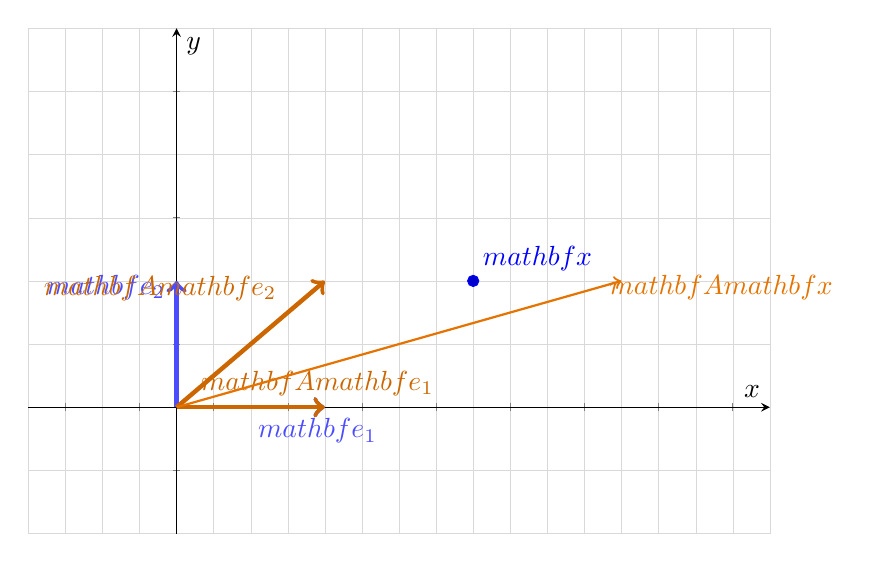
\begin{tikzpicture}
  \begin{axis}[
      axis lines=middle,
      xmin=-1, xmax=4,
      ymin=-1, ymax=3,
      xlabel={$x$}, ylabel={$y$},
      ticks=none,
      grid=both,
      minor tick num=1,
      grid style={line width=0.1pt, draw=gray!30},
      clip=false,
      width=11cm, height=8cm
  ]
    % original basis vectors
    \addplot[->, ultra thick, blue!70] coordinates {(0,0) (1,0)} node[pos=0.95, below] {$\\mathbf{e}_1$};
    \addplot[->, ultra thick, blue!70] coordinates {(0,0) (0,1)} node[pos=0.95, left] {$\\mathbf{e}_2$};

    % transformed basis for shear matrix [[1,1],[0,1]]
    \addplot[->, ultra thick, orange!80!black] coordinates {(0,0) (1,0)} node[pos=0.95, above] {$\\mathbf{A}\\mathbf{e}_1$};
    \addplot[->, ultra thick, orange!80!black] coordinates {(0,0) (1,1)} node[pos=0.75, above left] {$\\mathbf{A}\\mathbf{e}_2$};

    % sample vector and its transform
    \addplot+[only marks, mark=*] coordinates {(2,1)} node[above right] {$\\mathbf{x}$};
    \addplot[->, thick, orange!90!black] coordinates {(0,0) (3,1)} node[pos=0.95, right] {$\\mathbf{A}\\mathbf{x}$};
  \end{axis}
\end{tikzpicture}
\end{document}
